\onehalfspacing
\section{Đề số 25}
\graphicspath{{./img/}}
\begin{bt} 
    \hfill
   \begin{enumerate}[a.]
    \item Tính: $\mathrm{A}=1 \frac{13}{15} \cdot(0,5)^2 \cdot 3+\left(\frac{8}{15}-1 \frac{19}{60}\right): 1 \frac{23}{24}$
    \item So sánh: $16^{20}$ và $2^{100}$
   \end{enumerate}
\loigiai{
    \begin{enumerate}
        \item Biến đổi:\\[5px] 
        $A=\frac{7}{5}-\frac{47}{60}: \frac{47}{24}$\\[5px]
        $=\frac{7}{5}-\frac{2}{5} \\[5px]
        =1$
        \item Biến đổi: $16^{20}=2^{4.20}=2^{80}$\\[5px]
        + Có $2^{80}<2^{100}$ vì $(1<2 ; 80<100)$\\[5px]
        Vậy $16^{20}<2^{100}$
    \end{enumerate}
}
\end{bt}

\begin{bt}
    \hfill
	\begin{enumerate}[a.]
        \item Tìm $x$ biết: $|2 x-7|+\frac{1}{2}=1 \frac{1}{2}$
        \item Tìm số tự nhiên $\mathrm{n}$ biết: $3^{-1} \cdot 3^n+4.3^n=13.3^5$
    \end{enumerate}
	\loigiai{
        \begin{enumerate}
            \item + Ta có $|2 x-7|+\frac{1}{2}=1 \frac{1}{2} \Rightarrow|2 x-7|=1 \\[5px]
                \Rightarrow 2 x-7=1 \text { hoặc } 2 x-7=-1 \\[5px]
                \Rightarrow x=4 \text { hoặc } x=3 \\[5px]
                \text {Vậy } x=4 \text { hoặc } x=3.$
            \item + Biến đổi được $3^n \cdot\left(3^{-1}+4\right)=13 \cdot 3^5 \\[5px]
                \Rightarrow 3^n=3^6 \\[5px]
                \Rightarrow \mathrm{n}=6 \\[5px]
                \text {KL: Vậy } \mathrm{n}=6$
        \end{enumerate}
    } 
\end{bt}

\begin{bt}
    \hfill
    \begin{enumerate}[a.]
        \item Cho dãy tỉ số bằng nhau: $\frac{2 a+b+c+d}{a}=\frac{a+2 b+c+d}{b}=\frac{a+b+2 c+d}{c}=\frac{a+b+c+2 d}{d}$ Tính giá trị biểu thức $\mathrm{Q}$, biết $\mathrm{Q}=\frac{a+b}{c+d}+\frac{b+c}{d+a}+\frac{c+d}{a+b}+\frac{d+a}{b+c}$
        \item Cho biểu thức $M=\frac{x}{x+y+z}+\frac{y}{x+y+t}+\frac{z}{y+z+t}+\frac{t}{x+z+t}$ với $x, y, z$, t là các số tự nhiên khác 0 . Chứng minh $M^{10}<1025$.
    \end{enumerate}
	\loigiai{
        \begin{enumerate}
            \item Biến đổi: $\frac{2 a+b+c+d}{a}=\frac{a+2 b+c+d}{b}=\frac{a+b+2 c+d}{c}=\frac{a+b+c+2 d}{d} \\[5px]
            \frac{2 a+b+c+d}{a}-1=\frac{a+2 b+c+d}{b}-1=\frac{a+b+2 c+d}{c}-1=\frac{a+b+c+2 d}{d}-1 \\[5px]
            \frac{a+b+c+d}{a}=\frac{a+b+c+d}{b}=\frac{a+b+c+d}{c}=\frac{a+b+c+d}{d} \\[5px]
            + \text {Nếu } \mathrm{a}+\mathrm{b}+\mathrm{c}+\mathrm{d} \neq 0 \text { thì } \mathrm{a}=\mathrm{b}=\mathrm{c}=\mathrm{d}=>\mathrm{Q}=1+1+1+1=4 \\[5px]
            + \text {Nếu } \mathrm{a}+\mathrm{b}+\mathrm{c}+\mathrm{d}=0 \\[5px]
            \text {thì } \mathrm{a}+\mathrm{b}=-(\mathrm{c}+\mathrm{d}) ; \mathrm{b}+\mathrm{c}=-(\mathrm{d}+\mathrm{a}) ; \mathrm{c}+\mathrm{d}=-(\mathrm{a}+\mathrm{b}) ; \mathrm{d}+\mathrm{a}=-(\mathrm{b}+\mathrm{c}) \\[5px]
            \quad \Rightarrow \mathrm{Q}=(-1)+(-1)+(-1)+(-1)=-4 \\[5px]
            \mathrm{KL}: \text {Vậy } \mathrm{Q}=4 \text{ khi } \mathrm{a}+\mathrm{b}+\mathrm{c}+\mathrm{d} \neq 0 \\[5px]
            \quad \mathrm{Q}=-4 \text{ khi } \mathrm{a}+\mathrm{b}+\mathrm{c}+\mathrm{d}=0$
            \item Ta có: $\frac{x}{x+y+z}<\frac{x}{x+y} \\[5px]
            \frac{y}{x+y+t}<\frac{y}{x+y}
            \frac{z}{y+z+t}<\frac{z}{z+t} \\[5px]
            \frac{t}{x+z+t}<\frac{t}{z+t} \\[5px]
            \Rightarrow \mathrm{M}<\left(\frac{\mathrm{x}}{\mathrm{x}+\mathrm{y}}+\frac{\mathrm{y}}{\mathrm{x}+\mathrm{y}}\right)+\left(\frac{\mathrm{z}}{\mathrm{z}+\mathrm{t}}+\frac{\mathrm{t}}{\mathrm{z}+\mathrm{t}}\right) \Rightarrow \mathrm{M}<2 \\[5px]
             + \text {Có } \mathrm{M}^{10}<2^{10}(\text{Vì } M>0) \text { mà } 2^{10}=1024<1025 \\[5px]
            \text {Vậy } \mathrm{M}^{10}<1025$
        \end{enumerate}
    }
\end{bt}

\begin{bt}
    \hfill
    \begin{enumerate}[1)]
        \item Cho tam giác $\mathrm{ABC}$ vuông cân tại $\mathrm{A}$. Gọi $M$ là trung điểm $\mathrm{BC}, \mathrm{D}$ là điểm thuộc đoạn $\mathrm{BM}$ ( $\mathrm{D}$ khác $\mathrm{B}$ và $\mathrm{M})$. Kẻ các đường thẳng $\mathrm{BH}, \mathrm{CI}$ lần lượt vuông góc với đường thẳng $\mathrm{AD}$ tại $\mathrm{H}$ và $\mathrm{I}$. Chứng minh rằng:
        \begin{enumerate}[a.]
            \item $\mathrm{BAM}=\mathrm{ACM}$ và $\mathrm{BH}=\mathrm{AI}$.
            \item Tam giác MHI vuông cân.
        \end{enumerate}
        \item Cho tam giác $\mathrm{ABC}$ có góc $\widehat{\mathrm{A}}=90^{\circ}$. Kẻ $\mathrm{AH}$ vuông góc với $\mathrm{BC}$ (H thuộc $\left.\mathrm{BC}\right)$. Tia phân giác của góc $\mathrm{HAC}$ cắt cạnh $\mathrm{BC}$ ở điểm $\mathrm{D}$ và tia phân giác của góc $\mathrm{HAB}$ cắt cạnh $\mathrm{BC}$ ở $\mathrm{E}$. Chứng minh rằng $\mathrm{AB}+\mathrm{AC}=\mathrm{BC}+\mathrm{DE}$.
    \end{enumerate}
	\loigiai{
        $$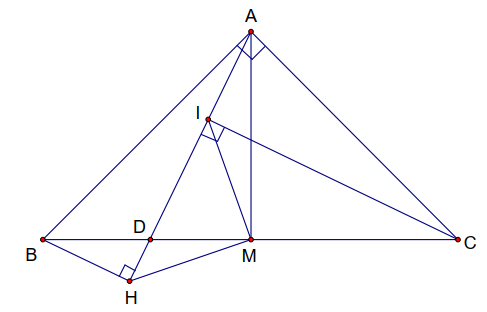
\includegraphics[width=0.5\textwidth]{25-4-lg.png}$$
        \begin{enumerate}[1.]
            \item \hfill
            \begin{enumerate}[a.]
                \item $*$ Chứng minh: $B A M=A C M$\\[5px]
                + Chứng minh được: $\triangle \mathrm{ABM}=\triangle \mathrm{ACM}(\mathrm{c}-\mathrm{c}-\mathrm{c})$\\[5px]
                + Lập luận được: $B A M=C A M=45^{\circ}$\\[5px]
                + Tính ra được $A C M=45^{\circ}$\\[5px]
                $\Rightarrow B A M=A C M$\\[5px]
                * Chứng minh: $\mathrm{BH}=\mathrm{AI}$.\\[5px]
                + Chỉ ra: $B A H=A C I$ (cùng phụ $D A C$ )\\[5px]
                + Chứng minh được $\triangle \mathrm{AIC}=\Delta \mathrm{BHA}$ (Cạnh huyên - góc nhọn)\\[5px]
                $\Rightarrow \mathrm{BH}=\mathrm{AI}$ (2 cạnh tương ứng)
                \item Tam giác MHI vuông cân.\\[5px]
                + Chứng minh được $A M \perp B C$\\[5px]
                + Chứng minh được $\mathrm{AM}=\mathrm{MC}$\\[5px]
                + Chứng minh được $H A M=I C M$\\[5px]
                + Chứng minh được $\Delta \mathrm{HAM}=\Delta \mathrm{ICM}(\mathrm{c}-\mathrm{g}-\mathrm{c})$\\[5px]
                $\Rightarrow \mathrm{HM}=\mathrm{MI}$(*)\\[5px]
                $\text {+ Do } \triangle \mathrm{HAM}=\triangle \mathrm{ICM} \Rightarrow H M A=I M C \Rightarrow H M B=I M A \text { (do } A M B=A M C=90^{\circ} \\[5px]
                \text {+ Lập luận được: } H M I=90^{\circ} \\[5px]
                \qquad \text {Từ }\left(^*\right) \text { và }\left({ }^{* *}\right)=>\Delta \mathrm{MHI} \text { vuông cân }$(**)\\[5px]
                Từ $\left({ }^*\right)$ và $\left({ }^{* *}\right)=>\Delta \mathrm{MHI}$ vuông cân
            \end{enumerate}
            \item \hfill 
            $$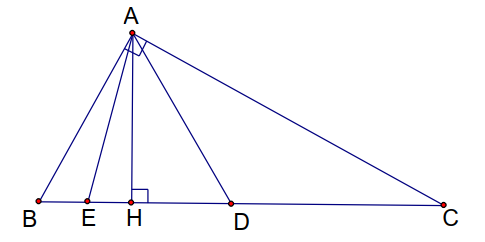
\includegraphics[width=0.5\textwidth]{25-4.2-lg.png}$$
            + Chứng minh được :\\[5px]
            $A E \mathrm{C}=A B C+B A E=H A D+D A C+B A E=E A H+H A D+D A C=E A C$\\[5px]
            (Vì $B$ và $H A C$ cùng phụ với $B A H$ )\\[5px]
            Suy ra tam giác $\mathrm{AEC}$ cân tại $\mathrm{C} \Rightarrow \mathrm{AC}=\mathrm{CE}$ (*)\\[5px]
            + Tương tự chứng minh được $\mathrm{AB}=\mathrm{BD}$
            $\left({ }^{* *}\right)$\\[5px]
            $+ \text { Từ }\left({ }^*\right) \text { và }\left({ }^{* *}\right) \Rightarrow \mathrm{AB}+\mathrm{AC}=\mathrm{BD}+\mathrm{EC}=\mathrm{ED}+\mathrm{BC}$
        \end{enumerate}
    }
\end{bt}

\begin{bt}
    Cho $\mathrm{x}, \mathrm{y}, \mathrm{z}$ là 3 số thực tùy ý thỏa mãn $\mathrm{x}+\mathrm{y}+\mathrm{z}=0$ và $-1 \leq x \leq 1$, $-1 \leq y \leq 1,$
    
    $-1 \leq z \leq 1$. Chứng minh rằng đa thức $x^2+y^4+z^6$ có giá trị không lớn hơn 2 .
\loigiai{
    +) Trong ba số $x, y, z$ có ít nhất hai số cùng dấu. Giả sử $x ; y \geq 0$\\[5px]
    $\Rightarrow \mathrm{z}=-\mathrm{x}-\mathrm{y} \leq 0 \\[5px]
    + \text { Vi }-1 \leq x \leq 1,-1 \leq y \leq 1,-1 \leq z \leq 1=>x^2+y^4+z^6 \leq|x|+|y|+|z| \\[5px]
    \Rightarrow x^2+y^4+z^6 \leq x+y-z \\[5px]
    \Rightarrow x^2+y^4+z^6 \leq-2 z \\[5px]
    +)-1 \leq z \leq 1 \text { và } \mathrm{z} \leq 0 \Rightarrow x^2+y^4+z^6 \leq 2 \\[5px]
    \text {KL: Vậy } x^2+y^4+z^6 \leq 2$
}
\end{bt}


